%%%%%%%%%%%%%%%%%%%%%%%%%%%%%%%%%%%%%%%%%%%%%%%%%%%%%%%%%%%%%%%%%%%%%%%%%%%%%%%%
%  IRIS 2027 (Shaastra, IIT Madras) -- final paper, Springer LNEE proceedings
%  Class: svproc (Springer Proceedings LaTeX2e package, v1.3). Do NOT edit svproc.cls.
%  Build: pdflatex main && pdflatex main      (no BibTeX needed: references are inline)
%
%  Every number comes from an auto-generated file -- never type results by hand:
%    generated_pilot.tex, generated_pilot_table.tex   <- paper/scripts/pilot.py  (audit, all 1,500 accident clips)
%    generated_eval.tex, generated_tab_{main,control,leak}.tex <- experiments/exp3_ccd/04_anticipation_eval.py
%    generated_within.tex, generated_tab_within.tex   <- experiments/exp3_ccd/06_within_clip.py
%    generated_extra.tex                              <- experiments/exp3_ccd/09_extra_macros.py
%    generated_runtime.tex                            <- experiments/exp3_ccd/08_runtime.py
%  Check before submission:  python scripts/check_paper.py
%%%%%%%%%%%%%%%%%%%%%%%%%%%%%%%%%%%%%%%%%%%%%%%%%%%%%%%%%%%%%%%%%%%%%%%%%%%%%%%%
\documentclass{svproc}
\usepackage{url}
\def\UrlFont{\rmfamily}
\usepackage{graphicx}
\usepackage{amsmath}
\usepackage{booktabs}
\newif\ifEvalAvailable \EvalAvailablefalse
% AUTO-GENERATED by pilot.py from the full CCD accident-clip run. Do not edit by hand.
\newcommand{\PilotN}{1500}
\newcommand{\PilotFrames}{75000}
\newcommand{\PilotDay}{1325}
\newcommand{\PilotNight}{175}
\newcommand{\PilotNormalW}{1141}
\newcommand{\PilotSnow}{235}
\newcommand{\PilotRain}{124}
\newcommand{\PilotEgo}{801}
\newcommand{\PilotOnsetMed}{3.6}
\newcommand{\PilotOnsetMin}{3.0}
\newcommand{\PilotOnsetMax}{4.9}
\newcommand{\LaneRate}{9.3}
\newcommand{\LaneRateRain}{8.3}
\newcommand{\LaneRateSnow}{4.3}
\newcommand{\LaneRateNormal}{10.4}
\newcommand{\LaneClipsAny}{37}
\newcommand{\TTCClipsAny}{1195}
\newcommand{\AlertEarly}{11.2}
\newcommand{\AlertMid}{11.5}
\newcommand{\AlertLate}{10.9}
\newcommand{\TDetN}{1500}
\newcommand{\TDetEarly}{1}
\newcommand{\TDetLate}{0.7}
\newcommand{\TDetDiff}{+0}
\newcommand{\TDetLo}{-0.1}
\newcommand{\TDetHi}{0}
\newcommand{\TDetInc}{8}
\newcommand{\TDetDec}{48}
\newcommand{\TDetP}{$<$0.001}
\newcommand{\TTTCN}{1500}
\newcommand{\TTTCEarly}{0.5}
\newcommand{\TTTCLate}{0.1}
\newcommand{\TTTCDiff}{+0}
\newcommand{\TTTCLo}{0}
\newcommand{\TTTCHi}{0}
\newcommand{\TTTCInc}{21}
\newcommand{\TTTCDec}{43}
\newcommand{\TTTCP}{$<$0.001}
\newcommand{\TVehN}{1500}
\newcommand{\TVehEarly}{2.4}
\newcommand{\TVehLate}{1}
\newcommand{\TVehDiff}{-0.9}
\newcommand{\TVehLo}{-1}
\newcommand{\TVehHi}{-0.8}
\newcommand{\TVehInc}{16}
\newcommand{\TVehDec}{74}
\newcommand{\TVehP}{$<$0.001}
\newcommand{\TFlowN}{1500}
\newcommand{\TFlowEarly}{1.14}
\newcommand{\TFlowLate}{1.75}
\newcommand{\TFlowDiff}{+0.427}
\newcommand{\TFlowLo}{0.347}
\newcommand{\TFlowHi}{0.536}
\newcommand{\TFlowInc}{70}
\newcommand{\TFlowDec}{30}
\newcommand{\TFlowP}{$<$0.001}
\newcommand{\TOccN}{1500}
\newcommand{\TOccEarly}{0.0189}
\newcommand{\TOccLate}{0.00868}
\newcommand{\TOccDiff}{-0.00334}
\newcommand{\TOccLo}{-0.00434}
\newcommand{\TOccHi}{-0.00259}
\newcommand{\TOccInc}{30}
\newcommand{\TOccDec}{63}
\newcommand{\TOccP}{$<$0.001}
\newcommand{\TInvTTCN}{1500}
\newcommand{\TInvTTCEarly}{0.231}
\newcommand{\TInvTTCLate}{0.0291}
\newcommand{\TInvTTCDiff}{+0}
\newcommand{\TInvTTCLo}{0}
\newcommand{\TInvTTCHi}{0}
\newcommand{\TInvTTCInc}{33}
\newcommand{\TInvTTCDec}{39}
\newcommand{\TInvTTCP}{0.01}
\newcommand{\TDistN}{824}
\newcommand{\TDistEarly}{16.1}
\newcommand{\TDistLate}{16}
\newcommand{\TDistDiff}{-0.0473}
\newcommand{\TDistLo}{-0.335}
\newcommand{\TDistHi}{0.183}
\newcommand{\TDistInc}{50}
\newcommand{\TDistDec}{50}
\newcommand{\TDistP}{0.97}
\newcommand{\TSharpN}{1500}
\newcommand{\TSharpEarly}{593}
\newcommand{\TSharpLate}{575}
\newcommand{\TSharpDiff}{-7.66}
\newcommand{\TSharpLo}{-11.7}
\newcommand{\TSharpHi}{-3.78}
\newcommand{\TSharpInc}{45}
\newcommand{\TSharpDec}{55}
\newcommand{\TSharpP}{$<$0.001}
\newcommand{\TBrightN}{1500}
\newcommand{\TBrightEarly}{0.446}
\newcommand{\TBrightLate}{0.442}
\newcommand{\TBrightDiff}{-0.00365}
\newcommand{\TBrightLo}{-0.00503}
\newcommand{\TBrightHi}{-0.0028}
\newcommand{\TBrightInc}{42}
\newcommand{\TBrightDec}{58}
\newcommand{\TBrightP}{$<$0.001}
\newcommand{\TGlareN}{1500}
\newcommand{\TGlareEarly}{0.00814}
\newcommand{\TGlareLate}{0.0088}
\newcommand{\TGlareDiff}{-6.36e-05}
\newcommand{\TGlareLo}{-0.000107}
\newcommand{\TGlareHi}{-3.73e-05}
\newcommand{\TGlareInc}{43}
\newcommand{\TGlareDec}{56}
\newcommand{\TGlareP}{$<$0.001}
\newcommand{\TDarkN}{1500}
\newcommand{\TDarkEarly}{0.298}
\newcommand{\TDarkLate}{0.291}
\newcommand{\TDarkDiff}{-0.00462}
\newcommand{\TDarkLo}{-0.0059}
\newcommand{\TDarkHi}{-0.00345}
\newcommand{\TDarkInc}{41}
\newcommand{\TDarkDec}{59}
\newcommand{\TDarkP}{$<$0.001}
\newcommand{\TContrastN}{1500}
\newcommand{\TContrastEarly}{0.25}
\newcommand{\TContrastLate}{0.25}
\newcommand{\TContrastDiff}{+0.000486}
\newcommand{\TContrastLo}{-0.000141}
\newcommand{\TContrastHi}{0.00111}
\newcommand{\TContrastInc}{52}
\newcommand{\TContrastDec}{48}
\newcommand{\TContrastP}{0.15}
\newcommand{\TDivN}{1500}
\newcommand{\TDivEarly}{0.0207}
\newcommand{\TDivLate}{0.0216}
\newcommand{\TDivDiff}{-2.2e-05}
\newcommand{\TDivLo}{-0.000602}
\newcommand{\TDivHi}{0.000742}
\newcommand{\TDivInc}{50}
\newcommand{\TDivDec}{50}
\newcommand{\TDivP}{0.49}
\newcommand{\TVRUN}{1500}
\newcommand{\TVRUEarly}{0}
\newcommand{\TVRULate}{0}
\newcommand{\TVRUDiff}{+0}
\newcommand{\TVRULo}{0}
\newcommand{\TVRUHi}{0}
\newcommand{\TVRUInc}{7}
\newcommand{\TVRUDec}{16}
\newcommand{\TVRUP}{$<$0.001}

% AUTO-GENERATED by 04_anticipation_eval.py -- do not edit by hand.
\EvalAvailabletrue
\def\EvalNCrash{1500}
\def\EvalNNormal{3000}
\def\EvalNTrain{3600}
\def\EvalNTest{900}
\def\EvalNTestCrash{300}
\def\EvalNTestNormal{600}
\def\EvalSplit{official CCD lists (train.txt/test.txt)}
\def\EvalFAR{10}
\def\EvalHorizon{2.0}
\def\LeakNuisAUC{1.00}
\def\LeakNuisLo{1.00}
\def\LeakNuisHi{1.00}
\def\LeakMNuisAUC{0.50}
\def\LeakMNuisLo{0.50}
\def\LeakMNuisHi{0.50}
\def\LeakSceneAUC{0.93}
\def\LeakSceneLo{0.91}
\def\LeakSceneHi{0.95}
\def\LeakMSceneAUC{0.50}
\def\LeakMSceneLo{0.50}
\def\LeakMSceneHi{0.50}
\def\LeakKinAUC{0.73}
\def\LeakKinLo{0.70}
\def\LeakKinHi{0.77}
\def\LeakMKinAUC{0.50}
\def\LeakMKinLo{0.50}
\def\LeakMKinHi{0.50}
\def\LeakMotionAUC{0.70}
\def\LeakMotionLo{0.66}
\def\LeakMotionHi{0.73}
\def\LeakMMotionAUC{0.50}
\def\LeakMMotionLo{0.50}
\def\LeakMMotionHi{0.50}
\def\LeakAllAUC{0.96}
\def\LeakAllLo{0.95}
\def\LeakAllHi{0.97}
\def\LeakMAllAUC{0.50}
\def\LeakMAllLo{0.50}
\def\LeakMAllHi{0.50}
\def\LeakVisNuisAUC{1.00}
\def\LeakVisNuisLo{1.00}
\def\LeakVisNuisHi{1.00}
\def\LeakMVisNuisAUC{0.50}
\def\LeakMVisNuisLo{0.50}
\def\LeakMVisNuisHi{0.50}
\def\RuleTunedAP{0.40}
\def\RuleTunedAPLo{0.36}
\def\RuleTunedAPHi{0.44}
\def\RuleTunedAUC{0.57}
\def\RuleTunedRecall{16}
\def\RuleTunedmTTA{2.23}
\def\RuleTunedRecallLo{12}
\def\RuleTunedRecallHi{19}
\def\RuleTunedFAR{10}
\def\RuleFixedAP{0.40}
\def\RuleFixedAPLo{0.36}
\def\RuleFixedAPHi{0.44}
\def\RuleFixedAUC{0.57}
\def\RuleFixedRecall{49}
\def\RuleFixedmTTA{2.27}
\def\RuleFixedRecallLo{43}
\def\RuleFixedRecallHi{54}
\def\RuleFixedFAR{34}
\def\RuleDivAP{0.39}
\def\RuleDivAPLo{0.36}
\def\RuleDivAPHi{0.43}
\def\RuleDivAUC{0.58}
\def\RuleDivRecall{14}
\def\RuleDivmTTA{1.35}
\def\RuleDivRecallLo{10}
\def\RuleDivRecallHi{18}
\def\RuleDivFAR{9}
\def\SceneAP{0.91}
\def\SceneAPLo{0.89}
\def\SceneAPHi{0.93}
\def\SceneAUC{0.95}
\def\SceneRecall{88}
\def\ScenemTTA{3.20}
\def\SceneRecallLo{84}
\def\SceneRecallHi{91}
\def\SceneFAR{12}
\def\KinAP{0.79}
\def\KinAPLo{0.75}
\def\KinAPHi{0.83}
\def\KinAUC{0.87}
\def\KinRecall{62}
\def\KinmTTA{1.96}
\def\KinRecallLo{56}
\def\KinRecallHi{67}
\def\KinFAR{10}
\def\MotionAP{0.66}
\def\MotionAPLo{0.61}
\def\MotionAPHi{0.71}
\def\MotionAUC{0.79}
\def\MotionRecall{44}
\def\MotionmTTA{1.29}
\def\MotionRecallLo{39}
\def\MotionRecallHi{50}
\def\MotionFAR{10}
\def\MotionTTCAP{0.47}
\def\MotionTTCAPLo{0.43}
\def\MotionTTCAPHi{0.53}
\def\MotionTTCAUC{0.67}
\def\MotionTTCRecall{23}
\def\MotionTTCmTTA{1.54}
\def\MotionTTCRecallLo{19}
\def\MotionTTCRecallHi{28}
\def\MotionTTCFAR{9}
\def\KinMotionAP{0.84}
\def\KinMotionAPLo{0.80}
\def\KinMotionAPHi{0.87}
\def\KinMotionAUC{0.90}
\def\KinMotionRecall{70}
\def\KinMotionmTTA{1.95}
\def\KinMotionRecallLo{64}
\def\KinMotionRecallHi{75}
\def\KinMotionFAR{9}
\def\FusedAP{0.97}
\def\FusedAPLo{0.96}
\def\FusedAPHi{0.98}
\def\FusedAUC{0.98}
\def\FusedRecall{95}
\def\FusedmTTA{2.92}
\def\FusedRecallLo{92}
\def\FusedRecallHi{97}
\def\FusedFAR{9}
\def\FusedMTTCAP{0.97}
\def\FusedMTTCAPLo{0.96}
\def\FusedMTTCAPHi{0.98}
\def\FusedMTTCAUC{0.98}
\def\FusedMTTCRecall{95}
\def\FusedMTTCmTTA{2.88}
\def\FusedMTTCRecallLo{93}
\def\FusedMTTCRecallHi{97}
\def\FusedMTTCFAR{10}
\def\FusedLRAP{0.89}
\def\FusedLRAPLo{0.85}
\def\FusedLRAPHi{0.93}
\def\FusedLRAUC{0.96}
\def\FusedLRRecall{86}
\def\FusedLRmTTA{2.74}
\def\FusedLRRecallLo{82}
\def\FusedLRRecallHi{90}
\def\FusedLRFAR{9}
\def\MRuleTunedAP{0.72}
\def\MRuleTunedAPLo{0.44}
\def\MRuleTunedAPHi{1.00}
\def\MRuleTunedAUC{0.67}
\def\MRuleTunedRecall{67}
\def\MRuleTunedmTTA{2.30}
\def\MRuleTunedRecallLo{0}
\def\MRuleTunedRecallHi{100}
\def\MRuleTunedFAR{33}
\def\MRuleFixedAP{0.72}
\def\MRuleFixedAPLo{0.44}
\def\MRuleFixedAPHi{1.00}
\def\MRuleFixedAUC{0.67}
\def\MRuleFixedRecall{33}
\def\MRuleFixedmTTA{0.40}
\def\MRuleFixedRecallLo{0}
\def\MRuleFixedRecallHi{100}
\def\MRuleFixedFAR{33}
\def\MRuleDivAP{0.92}
\def\MRuleDivAPLo{0.73}
\def\MRuleDivAPHi{1.00}
\def\MRuleDivAUC{0.89}
\def\MRuleDivRecall{100}
\def\MRuleDivmTTA{3.27}
\def\MRuleDivRecallLo{100}
\def\MRuleDivRecallHi{100}
\def\MRuleDivFAR{100}
\def\MSceneAP{0.92}
\def\MSceneAPLo{0.73}
\def\MSceneAPHi{1.00}
\def\MSceneAUC{0.89}
\def\MSceneRecall{67}
\def\MScenemTTA{2.50}
\def\MSceneRecallLo{0}
\def\MSceneRecallHi{100}
\def\MSceneFAR{0}
\def\MKinAP{0.56}
\def\MKinAPLo{0.43}
\def\MKinAPHi{1.00}
\def\MKinAUC{0.56}
\def\MKinRecall{100}
\def\MKinmTTA{2.87}
\def\MKinRecallLo{100}
\def\MKinRecallHi{100}
\def\MKinFAR{100}
\def\MMotionAP{0.63}
\def\MMotionAPLo{0.42}
\def\MMotionAPHi{1.00}
\def\MMotionAUC{0.33}
\def\MMotionRecall{100}
\def\MMotionmTTA{3.93}
\def\MMotionRecallLo{100}
\def\MMotionRecallHi{100}
\def\MMotionFAR{100}
\def\MMotionTTCAP{0.48}
\def\MMotionTTCAPLo{0.38}
\def\MMotionTTCAPHi{1.00}
\def\MMotionTTCAUC{0.33}
\def\MMotionTTCRecall{67}
\def\MMotionTTCmTTA{1.80}
\def\MMotionTTCRecallLo{0}
\def\MMotionTTCRecallHi{100}
\def\MMotionTTCFAR{67}
\def\MKinMotionAP{0.72}
\def\MKinMotionAPLo{0.44}
\def\MKinMotionAPHi{1.00}
\def\MKinMotionAUC{0.56}
\def\MKinMotionRecall{100}
\def\MKinMotionmTTA{3.03}
\def\MKinMotionRecallLo{100}
\def\MKinMotionRecallHi{100}
\def\MKinMotionFAR{100}
\def\MFusedAP{0.92}
\def\MFusedAPLo{0.73}
\def\MFusedAPHi{1.00}
\def\MFusedAUC{0.89}
\def\MFusedRecall{67}
\def\MFusedmTTA{2.55}
\def\MFusedRecallLo{0}
\def\MFusedRecallHi{100}
\def\MFusedFAR{0}
\def\MFusedMTTCAP{0.92}
\def\MFusedMTTCAPLo{0.73}
\def\MFusedMTTCAPHi{1.00}
\def\MFusedMTTCAUC{0.89}
\def\MFusedMTTCRecall{67}
\def\MFusedMTTCmTTA{2.55}
\def\MFusedMTTCRecallLo{0}
\def\MFusedMTTCRecallHi{100}
\def\MFusedMTTCFAR{0}
\def\MFusedLRAP{0.64}
\def\MFusedLRAPLo{0.43}
\def\MFusedLRAPHi{1.00}
\def\MFusedLRAUC{0.67}
\def\MFusedLRRecall{100}
\def\MFusedLRmTTA{3.93}
\def\MFusedLRRecallLo{100}
\def\MFusedLRRecallHi{100}
\def\MFusedLRFAR{33}
\def\DeltaAP{0.58}
\def\DeltaAPLo{0.53}
\def\DeltaAPHi{0.61}
\def\MDeltaAP{0.19}
\def\MDeltaAPLo{-0.17}
\def\MDeltaAPHi{0.50}
\def\DeltaAPKin{0.18}
\def\DeltaAPKinLo{0.15}
\def\DeltaAPKinHi{0.22}
\def\MDeltaAPKin{0.36}
\def\MDeltaAPKinLo{-0.17}
\def\MDeltaAPKinHi{0.57}
\def\DeltaAPMotion{0.31}
\def\DeltaAPMotionLo{0.26}
\def\DeltaAPMotionHi{0.36}
\def\MDeltaAPMotion{0.28}
\def\MDeltaAPMotionLo{-0.10}
\def\MDeltaAPMotionHi{0.58}
\def\DeltaAPScene{0.06}
\def\DeltaAPSceneLo{0.04}
\def\DeltaAPSceneHi{0.07}
\def\MDeltaAPScene{0.00}
\def\MDeltaAPSceneLo{0.00}
\def\MDeltaAPSceneHi{0.00}
\def\DeltaAPKinRule{0.39}
\def\DeltaAPKinRuleLo{0.33}
\def\DeltaAPKinRuleHi{0.44}
\def\MDeltaAPKinRule{-0.17}
\def\MDeltaAPKinRuleLo{-0.36}
\def\MDeltaAPKinRuleHi{0.00}
\def\DeltaAPMTTC{0.09}
\def\DeltaAPMTTCLo{0.03}
\def\DeltaAPMTTCHi{0.14}
\def\MDeltaAPMTTC{-0.44}
\def\MDeltaAPMTTCLo{-0.58}
\def\MDeltaAPMTTCHi{0.00}
\def\RuleTau{1.11}
\def\RuleDivTau{1.88}
\def\ShapKinematicShare{36}
\def\ShapMotionShare{16}
\def\ShapSceneShare{48}
\def\ShapMotionTtcShare{0}
\def\ShapTopOne{dark\_channel}
\def\ShapTopTwo{sharpness}
\def\ShapTopThree{n\_tracked}
\def\Frac720Crash{99}
\def\Frac720Normal{100}
\def\NuisTopFeat{file\_bytes}
\def\NuisTopAUC{0.04}
\def\DynFlowMagCenterAccidentLate{2.19}
\def\DynFlowMagCenterAccidentEarly{1.36}
\def\DynFlowMagCenterNormalLate{1.59}
\def\DynFlowMagCenterNormalEarly{1.53}
\def\DynHasDetAccidentLate{0.59}
\def\DynHasDetAccidentEarly{0.81}
\def\DynHasDetNormalLate{0.89}
\def\DynHasDetNormalEarly{0.90}
\def\DynMaxInvTtcPathAccidentLate{0.14}
\def\DynMaxInvTtcPathAccidentEarly{0.17}
\def\DynMaxInvTtcPathNormalLate{0.16}
\def\DynMaxInvTtcPathNormalEarly{0.16}
\def\MatchPairs{12}
\def\MatchPropAUC{1.00}
\def\MatchNCrash{12}
\def\MatchNNormal{12}
\def\MatchNTest{6}
\def\ShuffleAP{0.35}
\def\ShuffleAUC{0.51}
\def\ShufflePrev{0.34}
\def\SanityFARFused{9}
\def\CurveFusedRecallFarLo{92}
\def\CurveFusedmTTAFarLo{2.79}
\def\CurveFusedRecallFarHi{99}
\def\CurveFusedmTTAFarHi{3.37}
\def\CurveRuleTunedRecallFarLo{10}
\def\CurveRuleTunedmTTAFarLo{2.11}
\def\CurveRuleTunedRecallFarHi{37}
\def\CurveRuleTunedmTTAFarHi{2.20}
\def\CurveKinRecallFarLo{45}
\def\CurveKinmTTAFarLo{1.79}
\def\CurveKinRecallFarHi{86}
\def\CurveKinmTTAFarHi{2.30}
\def\SliceDayRecall{97}
\def\SliceDayRecallLo{95}
\def\SliceDayRecallHi{99}
\def\SliceDayAP{0.98}
\def\SliceDayN{264}
\def\SliceNightRecall{81}
\def\SliceNightRecallLo{67}
\def\SliceNightRecallHi{93}
\def\SliceNightAP{0.69}
\def\SliceNightN{36}
\def\SliceWNormalRecall{95}
\def\SliceWNormalRecallLo{93}
\def\SliceWNormalRecallHi{98}
\def\SliceWNormalAP{0.96}
\def\SliceWNormalN{228}
\def\SliceRainRecall{89}
\def\SliceRainRecallLo{74}
\def\SliceRainRecallHi{100}
\def\SliceRainAP{0.80}
\def\SliceRainN{19}
\def\SliceSnowRecall{96}
\def\SliceSnowRecallLo{91}
\def\SliceSnowRecallHi{100}
\def\SliceSnowAP{0.94}
\def\SliceSnowN{53}
\def\SliceEgoYesRecall{97}
\def\SliceEgoYesRecallLo{94}
\def\SliceEgoYesRecallHi{99}
\def\SliceEgoYesAP{0.97}
\def\SliceEgoYesN{158}
\def\SliceEgoNoRecall{93}
\def\SliceEgoNoRecallLo{89}
\def\SliceEgoNoRecallHi{97}
\def\SliceEgoNoAP{0.93}
\def\SliceEgoNoN{142}

% AUTO-GENERATED by 06_within_clip.py -- do not edit by hand.
\def\WNTest{300}
\def\WNTrain{1200}
\def\WRuleBoxAUC{0.45}
\def\WRuleBoxAUCLo{0.43}
\def\WRuleBoxAUCHi{0.48}
\def\WRuleBoxAP{0.37}
\def\WRuleBoxRecall{42}
\def\WRuleBoxRecallLo{36}
\def\WRuleBoxRecallHi{47}
\def\WRuleBoxmTTA{1.47}
\def\WRuleBoxFAR{11}
\def\WRuleDivAUC{0.56}
\def\WRuleDivAUCLo{0.54}
\def\WRuleDivAUCHi{0.59}
\def\WRuleDivAP{0.44}
\def\WRuleDivRecall{48}
\def\WRuleDivRecallLo{42}
\def\WRuleDivRecallHi{53}
\def\WRuleDivmTTA{1.27}
\def\WRuleDivFAR{10}
\def\WFlowMagAUC{0.67}
\def\WFlowMagAUCLo{0.65}
\def\WFlowMagAUCHi{0.70}
\def\WFlowMagAP{0.56}
\def\WFlowMagRecall{53}
\def\WFlowMagRecallLo{47}
\def\WFlowMagRecallHi{58}
\def\WFlowMagmTTA{1.09}
\def\WFlowMagFAR{8}
\def\WSceneAUC{0.80}
\def\WSceneAUCLo{0.77}
\def\WSceneAUCHi{0.82}
\def\WSceneAP{0.68}
\def\WSceneRecall{74}
\def\WSceneRecallLo{69}
\def\WSceneRecallHi{79}
\def\WScenemTTA{1.29}
\def\WSceneFAR{8}
\def\WKinAUC{0.87}
\def\WKinAUCLo{0.85}
\def\WKinAUCHi{0.89}
\def\WKinAP{0.74}
\def\WKinRecall{76}
\def\WKinRecallLo{71}
\def\WKinRecallHi{80}
\def\WKinmTTA{1.39}
\def\WKinFAR{6}
\def\WMotionAUC{0.79}
\def\WMotionAUCLo{0.76}
\def\WMotionAUCHi{0.81}
\def\WMotionAP{0.67}
\def\WMotionRecall{74}
\def\WMotionRecallLo{69}
\def\WMotionRecallHi{78}
\def\WMotionmTTA{1.16}
\def\WMotionFAR{9}
\def\WMotionTTCAUC{0.82}
\def\WMotionTTCAUCLo{0.80}
\def\WMotionTTCAUCHi{0.84}
\def\WMotionTTCAP{0.65}
\def\WMotionTTCRecall{87}
\def\WMotionTTCRecallLo{84}
\def\WMotionTTCRecallHi{91}
\def\WMotionTTCmTTA{1.47}
\def\WMotionTTCFAR{10}
\def\WKinMotionAUC{0.91}
\def\WKinMotionAUCLo{0.89}
\def\WKinMotionAUCHi{0.92}
\def\WKinMotionAP{0.82}
\def\WKinMotionRecall{89}
\def\WKinMotionRecallLo{86}
\def\WKinMotionRecallHi{92}
\def\WKinMotionmTTA{1.35}
\def\WKinMotionFAR{7}
\def\WFusedAUC{0.92}
\def\WFusedAUCLo{0.91}
\def\WFusedAUCHi{0.93}
\def\WFusedAP{0.86}
\def\WFusedRecall{90}
\def\WFusedRecallLo{87}
\def\WFusedRecallHi{93}
\def\WFusedmTTA{1.39}
\def\WFusedFAR{7}

% AUTO-GENERATED by 09_extra_macros.py -- do not edit by hand.
\def\BitrateCrash{105}
\def\BitrateNormal{369}
\def\BitrateRatio{3.5}
\def\BppCrash{0.09}
\def\BppNormal{0.32}
\def\NoiseCrash{0.0}
\def\NoiseNormal{1.5}
\def\ResOtherCrash{35}
\def\ResOtherNormal{0}
\def\FrameDiffCrash{7.4}
\def\FrameDiffNormal{6.8}
\def\NFramesOtherNormal{2}
\def\BitrateOverlapCrash{25}
\def\BitrateOverlapNormal{15}
\def\CtrlFlowRrb{0.33}
\def\CtrlFlowP{$<$0.001}
\def\CtrlDetRrb{-0.37}
\def\CtrlDetP{$<$0.001}
\def\CtrlVehRrb{-0.41}
\def\CtrlVehP{$<$0.001}
\def\CtrlInvTTCRrb{-0.11}
\def\CtrlInvTTCP{$<$0.001}
\def\CtrlDivPRrb{0.32}
\def\CtrlDivPP{$<$0.001}
\def\MatchPairs{12}
\def\MatchPropAUC{1.000}

% AUTO-GENERATED by 08_runtime.py
\def\RtDetect{44}
\def\RtScene{21}
\def\RtFlow{30}
\def\RtLane{5}
\def\RtKin{0.4}
\def\RtTotal{100}
\def\RtFPS{10}
\def\RtFPSNoLane{10}
\def\RtDevice{NVIDIA GeForce RTX 4060 Laptop GPU}


\begin{document}
\mainmatter
\title{DriveSense: An Explainable Baseline for Early Collision Anticipation from Dashcam Video Using Calibration-Free Cues}
\titlerunning{DriveSense: Explainable Collision Anticipation from Dashcam Video}
% Authors: order + corresponding author must match the Contributor Agreement and the e-mail exactly.
\author{Siddhi Dhoke\thanks{Corresponding author.} \and Nakul Bhadade}
\authorrunning{S. Dhoke and N. Bhadade}
\institute{Indian Institute of Information Technology Nagpur, Nagpur, Maharashtra, India\\
\email{sidii0080@gmail.com, nakulccs@gmail.com}}
\maketitle

\begin{abstract}
Anticipating a collision from a single forward camera is central to low-cost driver assistance, yet anticipation models are mostly opaque and are benchmarked on accident and normal clips that come from different video sources. We present DriveSense, a lightweight, explainable baseline for early collision anticipation from dashcam video, and use it to audit the Car Crash Dataset. It combines YOLOv8 detection with ByteTrack tracking, a calibration-free time-to-contact cue from the growth of tracked boxes, a detector-free time-to-contact from optical-flow divergence, photometric scene descriptors and central flow, fused by gradient-boosted trees with TreeSHAP attributions. We split by clip with the official lists, fix thresholds on held-out clips and report bootstrap confidence intervals. On the first second of each clip, before any accident, encoding properties alone separate accident from normal clips with an AUC of \LeakNuisAUC{}, and visual cues with \LeakAllAUC; the fused model's crash-versus-normal average precision of \FusedAP{} therefore cannot be read as anticipation skill. Comparing frames within accident clips removes the source: fused cues separate the last second before the accident from frames over two seconds earlier with an AUC of \WFusedAUC{} (95\% CI [\WFusedAUCLo, \WFusedAUCHi]), kinematic cues alone reach \WKinAUC, and the box-growth time-to-contact rule is no better than chance (\WRuleBoxAUC). Detector coverage falls toward impact, whereas detector-free flow magnitude rises in \TFlowInc\% of accident clips and not in normal clips.
\keywords{Collision anticipation, Dashcam video, Time-to-contact, Explainable AI, Dataset source bias, Monocular vision}
\end{abstract}

%=============================================================================
\section{Introduction}
%=============================================================================
Road traffic crashes kill about 1.19 million people every year~\cite{who2023}. Single-camera forward collision warning is attractive where radar-equipped vehicles are rare. The research community frames the problem as \emph{accident anticipation}: raise an alert as early as possible before an accident while keeping false alarms low~\cite{chan2016,suzuki2018,bao2020}. Recent deep, end-to-end models reach high average precision, but their alerts are hard to inspect, and they are usually trained and tested on accident and normal clips from different video sources. If those sources differ in resolution, compression, camera placement or weather, a classifier can separate them without modeling risk at all---a form of dataset bias or shortcut learning~\cite{torralba2011,geirhos2020}. A lightweight, interpretable baseline can expose such effects, because every alert traces to named, physically meaningful cues.

We present \emph{DriveSense}, an explainable anticipation baseline for monocular dashcam video, with three contributions:
\begin{enumerate}
\item Two \textbf{calibration-free time-to-contact (TTC) cues}, one from the growth of tracked boxes and one, detector-free, from optical-flow divergence, with an audit of their availability in accident footage.
\item A \textbf{source-leakage test} showing how much of the crash-versus-normal separation of the Car Crash Dataset is already present before any accident, and a \textbf{within-accident protocol} that removes the source difference by contrasting frames of the same clip.
\item An \textbf{explainable gradient-boosted baseline} with feature-group ablations, rule-based TTC baselines, metrics at a fixed false-alarm rate with bootstrap confidence intervals, and TreeSHAP attributions~\cite{lundberg2017,lundberg2020}.
\end{enumerate}

%=============================================================================
\section{Related Work}
%=============================================================================
Chan et al.~\cite{chan2016} introduced dashcam accident anticipation with a dynamic-spatial-attention recurrent network and the mean time-to-accident (mTTA) metric; Suzuki et al.~\cite{suzuki2018} proposed an adaptive loss for early anticipation; Bao et al.~\cite{bao2020} released the Car Crash Dataset (CCD) with a graph-recurrent Bayesian model; and Yao et al.~\cite{yao2023} studied unsupervised traffic anomaly detection on DoTA. These methods learn appearance features end-to-end, whereas we seek a transparent baseline in which each cue's contribution is measurable. The ratio of an object's image size to its rate of expansion specifies time-to-contact without distance or speed~\cite{lee1976}, a principle used by commercial monocular forward collision warning~\cite{dagan2004}; we apply it on top of a generic detector and tracker~\cite{yolov8,zhang2022} and use gradient-boosted trees~\cite{chen2016} with exact TreeSHAP~\cite{lundberg2020}.

%=============================================================================
\section{Method}
%=============================================================================
Figure~\ref{fig:pipeline} summarizes the pipeline; every cue is computed causally from current and past frames.

\begin{figure}[!t]
\centering
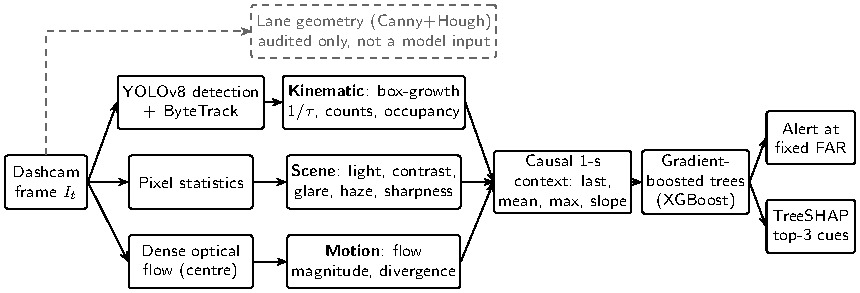
\includegraphics[width=0.8\textwidth]{figures/fig_pipeline.pdf}
\caption{DriveSense pipeline. Kinematic, scene and motion cues are summarized over a causal 1-s context and fused by gradient-boosted trees; TreeSHAP attributes each alert to its cues. Lane geometry is audited but not used as a model input}
\label{fig:pipeline}
\end{figure}

\subsection{Perception Front End}
YOLOv8-s~\cite{yolov8} detects cars, buses, trucks, motorcycles, bicycles and pedestrians (confidence $\geq 0.25$, input size 960 pixels), and ByteTrack~\cite{zhang2022} links detections into tracks; tracker state is reset at the start of each clip. A detection is \emph{in path} if its horizontal center lies within $\pm 0.22W$ of the image center and its bottom edge lies in the lower half of the frame, where $W$ is the image width.

\subsection{Calibration-Free Time-to-Contact}
Under a pinhole camera, an object of physical size $S$ at depth $Z(t)$ has image size $s(t)=fS/Z(t)$. Differentiating the logarithm removes both the focal length $f$ and the unknown size $S$:
\begin{equation}
\frac{\mathrm{d}\ln s}{\mathrm{d}t} = -\frac{\dot Z}{Z} = \frac{1}{\tau}, \qquad \tau = -\frac{Z}{\dot Z},
\label{eq:tau}
\end{equation}
where $\tau$ is the time-to-contact under constant closing speed~\cite{lee1976,dagan2004}. For each track we use $s=\sqrt{wh}$ for vehicles and $s=h$ for vulnerable road users, where $w$ and $h$ are the box width and height, and estimate $\widehat{\tau^{-1}}$ as the least-squares slope of $\ln s$ against time over the last 0.6~s (at least four samples). An object is treated as approaching when $\widehat{\tau^{-1}} > 0.02\,\mathrm{s}^{-1}$. The per-frame kinematic cue is the largest $\widehat{\tau^{-1}}$ among in-path tracks (and, separately, among all tracks); working with $1/\tau$ rather than $\tau$ keeps the cue bounded when nothing approaches.
\subsection{Scene, Motion and Lane Descriptors}
Per frame we compute brightness, contrast (gray-level standard deviation), glare fraction (pixels $\geq 245$), sharpness (Laplacian variance), a dark-channel haze proxy ($15\times15$ minimum filter) and saturation. Dense optical flow is computed with the Farneb\"ack method~\cite{farneback2003} (OpenCV; pyramid scale 0.5, 3 levels, window 15, 3 iterations, polynomial size 5, $\sigma=1.2$) between consecutive gray frames shrunk to a quarter of their size. Central flow magnitude and the flow divergence $D=\partial u/\partial x+\partial v/\partial y$ (flow in pixels per frame) are averaged over the central region (rows 40--90\%, columns 30--70\% of the frame), without any detector. For a surface approaching at constant speed the divergence equals $2/\tau$ per unit time, which gives a detector-free time-to-contact,
\begin{equation}
\tau_{\mathrm{div}} = \frac{2}{f_{\mathrm{s}}\,\max(\bar D,\epsilon)},
\label{eq:taudiv}
\end{equation}
with the frame rate $f_{\mathrm{s}}=10$ and $\tau_{\mathrm{div}}$ clipped to $[0.1,10]$~s; $1/\tau_{\mathrm{div}}$ and $\tau_{\mathrm{div}}$ form the \emph{motion-TTC} group. Lanes are detected with Canny edges and a Hough transform; because this failed on most accident clips (Sect.~\ref{sec:pilot}), lane cues are audited but not used by the models.

\subsection{Explainable Anticipation Model}
For every base cue $c$ we form four causal context features over the last second (10 frames): the current value, the mean, the maximum and the slope. Cues form four groups: \emph{kinematic} (box-growth $1/\tau$, object counts, box occupancy, detection and TTC availability), \emph{scene} (photometric), \emph{motion} (flow) and \emph{motion-TTC}. An XGBoost classifier~\cite{chen2016} (300 trees, depth 4, learning rate 0.05, class-balanced) is trained on frames: positive frames lie within \EvalHorizon~s before the annotated accident onset, negative frames are normal-clip frames, and earlier accident frames are excluded as ambiguous. An alert is raised the first time the score, averaged over the last three frames, exceeds a threshold $\theta$. TreeSHAP~\cite{lundberg2020} decomposes each score exactly as
\begin{equation}
g(\mathbf{x}_t) = \phi_0 + \sum_{i=1}^{M} \phi_i(\mathbf{x}_t),
\label{eq:shap}
\end{equation}
where $g$ is the log-odds output, $\phi_0$ its expectation and $\phi_i$ the contribution of feature $i$; summing over a cue's four context features gives cue-level attributions. The \emph{rule baselines} alert when the smoothed in-path $\widehat{\tau^{-1}}$ (or $1/\tau_{\mathrm{div}}$) exceeds a threshold, tuned like the models or, for boxes, fixed at $\tau<2$~s.

%=============================================================================
\section{Experimental Protocol}
%=============================================================================
\subsection{Data and Splits}
The Car Crash Dataset (CCD)~\cite{bao2020} contains 1,500 accident clips collected from YouTube and 3,000 normal clips sampled from BDD100K~\cite{yu2020}, each 5~s at 10 frames per second (50 frames); the accident onset frame, day or night, weather and ego-vehicle involvement are annotated for each accident clip. We use all \EvalNCrash{} accident and \EvalNNormal{} normal clips and the official training and test lists (\EvalNTrain{} training and \EvalNTest{} test clips, of which \EvalNTestCrash{} accident clips). Twenty percent of the training clips are held out to fix every threshold. Each normal clip receives a deterministic pseudo-onset drawn from the empirical accident-onset distribution, so both classes are scored over spans of equal length distribution.

\subsection{Metrics}
A clip's score is its maximum smoothed frame score before (pseudo-)onset, giving average precision (AP) and ROC-AUC over test clips. At the threshold giving a \EvalFAR\% false-alarm rate (FAR, share of normal clips with any alert) on held-out clips, we report test FAR, recall, mTTA (mean lead time of the first alert over alerted accident clips) and the share alerted $\geq$1~s ahead. 95\% confidence intervals (CIs) use 1,000 bootstrap resamples of clips.

\subsection{Leakage Test and Within-Accident Protocol}
\label{sec:within}
The leakage test summarizes each clip by the means of its cues over the first second (accident clips only if this ends $\geq$1~s before onset, which holds for all) and reports the test AUC of a classifier for accident versus normal. Besides scene, kinematic and motion cues we include \emph{encoding} cues that describe how a clip was stored rather than what it shows: file size and bits per pixel and second, resolution, a block-artifact measure, a noise estimate, letterbox borders and the mean frame difference. Because source differences can then explain any crash-versus-normal score, the \emph{within-accident protocol} uses accident clips only: frames more than 2~s before the onset are negatives, the last second before the onset is positive, and frames in between are ignored. Source, camera and encoder are shared by both classes, so a score can separate them only through what changes as the accident approaches. Thresholds are fixed on held-out training clips at a frame-level false-alarm rate of \EvalFAR\%; recall is the share of test accident clips alerted within the last 2~s.

\subsection{Control Comparison and Audit}
\label{sec:pilotprot}
The control comparison takes each cue's change from an early ($[-3,-2)$~s) to a late ($[-1,0)$~s) window relative to (pseudo-)onset and compares accident and normal clips with Mann--Whitney tests, Holm-corrected~\cite{holm1979}, with rank-biserial effect sizes ($r_{\mathrm{rb}}$) and bootstrap CIs~\cite{efron1993}. The audit applies the same windows to the \PilotN{} accident clips alone (\PilotDay{} day, \PilotNight{} night; \PilotNormalW{} normal weather, \PilotSnow{} snowy, \PilotRain{} rainy; onsets \PilotOnsetMin--\PilotOnsetMax~s) with paired Wilcoxon tests, Holm-corrected across 14 cues.

%=============================================================================
\section{Results}
%=============================================================================
\subsection{Audit: Which Cues Survive Accident Footage?}
\label{sec:pilot}
\paragraph{Lane markings and box-growth TTC are unreliable.} The lane detector found both boundaries in only \LaneRate\% of frames (\LaneRateSnow\% in snow) and in any frame at all in \LaneClipsAny\% of clips. The share of frames with any detection fell from a median of \TDetEarly{} in the early window to \TDetLate{} in the late window (decrease in \TDetDec\% of clips, Holm $p$ \TDetP), together with vehicle counts (\TVehEarly{} to \TVehLate). An in-path TTC estimate existed in some frame of \TTCClipsAny{} of \PilotN{} clips, but the largest in-path $1/\tau$ did not increase toward impact (median change \TInvTTCDiff~s$^{-1}$; increase in \TInvTTCInc\%, decrease in \TInvTTCDec\% of clips), and a rule alerting at $\tau<2$~s for an in-path object fired in \AlertEarly\% of early and \AlertLate\% of late frames. Box-based monocular cues thus do not strengthen when they are needed most.

\paragraph{A detector-free motion cue rises.} Central flow magnitude rose from \TFlowEarly{} to \TFlowLate{} (median change \TFlowDiff, 95\% CI [\TFlowLo, \TFlowHi]) and increased in \TFlowInc\% of clips (Holm $p$ \TFlowP). Photometric cues shifted by at most 3\% of their level (e.g., brightness \TBrightEarly{} to \TBrightLate), so the windows do not differ merely in lighting.

\subsection{Source Leakage}
Table~\ref{tab:leak} shows that the first second of a clip, before any accident, already reveals its class. Encoding cues alone give a test AUC of \LeakNuisAUC{} (95\% CI [\LeakNuisLo, \LeakNuisHi]): the median bit rate is \BitrateCrash~kB/s for accident clips and \BitrateNormal~kB/s for normal clips (a factor of \BitrateRatio), all normal clips have 1280$\times$720 pixels whereas \ResOtherCrash{} accident clips do not, and noise estimates differ (median \NoiseCrash{} versus \NoiseNormal). Scene cues alone reach \LeakSceneAUC{} [\LeakSceneLo, \LeakSceneHi], all visual cues \LeakAllAUC{} [\LeakAllLo, \LeakAllHi], and even the kinematic and motion cues reach \LeakKinAUC{} and \LeakMotionAUC. Part of the crash-versus-normal separability of CCD is therefore source-driven and independent of the accident. Pairing each accident clip with a normal clip of similar encoding is infeasible: the encoding classifier separates the classes almost perfectly (out-of-fold AUC \MatchPropAUC) and only \MatchPairs{} pairs fall within the matching caliper. We therefore treat crash-versus-normal results as confounded and rely on the within-accident protocol.

\begin{table}[!t]
\caption{Source leakage: test AUC of a classifier that sees only the first second of a clip, before any accident}
\label{tab:leak}
\centering\scriptsize
\setlength{\tabcolsep}{3pt}
% AUTO-GENERATED by 04_anticipation_eval.py
\begin{tabular}{@{}ll@{}}
\toprule
Cues from the first second only & Test AUC [95\% CI]\\
\midrule
Nuisance (encoding) only & 1.00 [1.00, 1.00]\\
Scene cues only & 0.93 [0.91, 0.95]\\
Kinematic cues only & 0.73 [0.70, 0.77]\\
Motion cues only & 0.70 [0.66, 0.73]\\
All visual cues & 0.96 [0.95, 0.97]\\
Visual + nuisance & 1.00 [1.00, 1.00]\\
\bottomrule
\end{tabular}

\end{table}

\subsection{Crash-Versus-Normal Anticipation}
Table~\ref{tab:main} reports test performance at a \EvalFAR\% false-alarm rate. The tuned TTC rule ($\tau=\RuleTau$~s) has an AP of \RuleTunedAP{} and recalls \RuleTunedRecall\% of accident clips; the fixed $\tau<2$~s rule alerts \RuleFixedRecall\% of accident clips but also \RuleFixedFAR\% of normal clips. The flow-divergence rule is comparable (AP \RuleDivAP). Learned models are far better: the fused model reaches an AP of \FusedAP{} (95\% CI [\FusedAPLo, \FusedAPHi]), recall \FusedRecall\% and mTTA \FusedmTTA~s, \DeltaAP{} AP above the tuned rule (95\% CI [\DeltaAPLo, \DeltaAPHi]). However, scene cues alone already reach an AP of \SceneAP{} and recall \SceneRecall\%, above kinematic cues (\KinAP) and motion cues (\MotionAP), and they dominate the TreeSHAP attribution of the fused model (\ShapSceneShare\% scene, \ShapKinematicShare\% kinematic, \ShapMotionShare\% motion; top cues \texttt{\ShapTopOne}, \texttt{\ShapTopTwo}, \texttt{\ShapTopThree}; attributions are additive and not causal). Together with Table~\ref{tab:leak}, this means these numbers mostly measure source recognition and should not be read as anticipation skill. Recall of the fused model rises from \CurveFusedRecallFarLo\% at a 5\% to \CurveFusedRecallFarHi\% at a 30\% false-alarm rate, against \CurveRuleTunedRecallFarLo\% to \CurveRuleTunedRecallFarHi\% for the box-TTC rule.

\begin{table}[!t]
\caption{Accident versus normal clips, CCD test set (confounded by source, Table~\ref{tab:leak}). AP and recall with 95\% CI, ROC-AUC, test false-alarm rate (FAR, \%), mTTA (s) of alerted clips and share alerted $\geq$1~s ahead (R@1s, \%); thresholds fixed at \EvalFAR\% FAR on held-out training clips. The two box-TTC rules share one score}
\label{tab:main}
\centering\scriptsize
\setlength{\tabcolsep}{3pt}
% AUTO-GENERATED by 04_anticipation_eval.py
\begin{tabular}{@{}llrrlrr@{}}
\toprule
Method & AP [95\% CI] & AUC & FAR & Recall [95\% CI] & mTTA & R@1s\\
\midrule
Rule: box-TTC (tuned) & 0.40 [0.36, 0.44] & 0.57 & 10 & 16 [12, 19] & 2.23 & 13\\
Rule: box-TTC $<$ 2 s (fixed) & 0.40 [0.36, 0.44] & 0.57 & 34 & 49 [43, 54] & 2.27 & 40\\
Rule: flow-divergence TTC (tuned) & 0.39 [0.36, 0.43] & 0.58 & 9 & 14 [10, 18] & 1.35 & 8\\
\midrule
Scene only & 0.91 [0.89, 0.93] & 0.95 & 12 & 88 [84, 91] & 3.20 & 84\\
Kinematic only & 0.79 [0.75, 0.83] & 0.87 & 10 & 62 [56, 67] & 1.96 & 54\\
Motion only & 0.66 [0.61, 0.71] & 0.79 & 10 & 44 [39, 50] & 1.29 & 22\\
Motion-TTC only & 0.47 [0.43, 0.53] & 0.67 & 9 & 23 [19, 28] & 1.54 & 16\\
Kinematic + motion & 0.84 [0.80, 0.87] & 0.90 & 9 & 70 [64, 75] & 1.95 & 59\\
Fused (all cues) & 0.97 [0.96, 0.98] & 0.98 & 9 & 95 [92, 97] & 2.92 & 93\\
Fused + motion-TTC & 0.97 [0.96, 0.98] & 0.98 & 10 & 95 [93, 97] & 2.88 & 93\\
Fused, logistic regression & 0.89 [0.85, 0.93] & 0.96 & 9 & 86 [82, 90] & 2.74 & 78\\
\bottomrule
\end{tabular}

\end{table}

\subsection{Within-Accident Anticipation}
Table~\ref{tab:within} compares frames of the same clips and so removes the source difference (\WNTest{} test accident clips). The box-growth rule is no better than chance (AUC \WRuleBoxAUC{} [\WRuleBoxAUCLo, \WRuleBoxAUCHi]): in accident footage the largest in-path $1/\tau$ does not rise as the accident approaches. The detector-free rule from flow divergence is weak but above chance (\WRuleDivAUC{} [\WRuleDivAUCLo, \WRuleDivAUCHi]), and learned models are much better: \WMotionTTCAUC{} for the motion-TTC cues alone, \WKinAUC{} for kinematic cues (detections, counts, box occupancy and box growth), \WMotionAUC{} for flow and \WSceneAUC{} for scene cues. Kinematic and motion cues are complementary (\WKinMotionAUC{}), and the fused model reaches an AUC of \WFusedAUC{} [\WFusedAUCLo, \WFusedAUCHi] and an AP of \WFusedAP{}, and alerts \WFusedRecall\% of test accident clips within the last 2~s at a \WFusedFAR\% frame-level false-alarm rate (mTTA \WFusedmTTA~s). Scene cues also separate the two phases (\WSceneAUC), as expected when the camera approaches an obstacle, so we do not read this group as risk-specific.

\begin{table}[!t]
\caption{Within-accident anticipation on \WNTest{} test accident clips: frames $>2$~s before the onset (negative) versus the last second (positive). Frame-level AUC and AP; recall of clips alerted within the last 2~s and mean lead time (s) at a \EvalFAR\% false-alarm rate on far frames; CIs bootstrapped over clips}
\label{tab:within}
\centering\scriptsize
\setlength{\tabcolsep}{3pt}
% AUTO-GENERATED by 06_within_clip.py
\begin{tabular}{@{}lllrr@{}}
\toprule
Score & AUC [95\% CI] & AP & Recall [95\% CI] & mTTA\\
\midrule
Rule: box-TTC & 0.45 [0.43, 0.48] & 0.37 & 42 [36, 47] & 1.47\\
Rule: flow-divergence TTC & 0.56 [0.54, 0.59] & 0.44 & 48 [42, 53] & 1.27\\
Flow magnitude (no learning) & 0.67 [0.65, 0.70] & 0.56 & 53 [47, 58] & 1.09\\
\midrule
Scene only & 0.80 [0.77, 0.82] & 0.68 & 74 [69, 79] & 1.29\\
Kinematic only & 0.87 [0.85, 0.89] & 0.74 & 76 [71, 80] & 1.39\\
Motion only & 0.79 [0.76, 0.81] & 0.67 & 74 [69, 78] & 1.16\\
Motion-TTC only & 0.82 [0.80, 0.84] & 0.65 & 87 [84, 91] & 1.47\\
Kinematic + motion & 0.91 [0.89, 0.92] & 0.82 & 89 [86, 92] & 1.35\\
Fused (all cues) & 0.92 [0.91, 0.93] & 0.86 & 90 [87, 93] & 1.39\\
\bottomrule
\end{tabular}

\end{table}

\subsection{Are Pre-Accident Changes Accident-Specific?}
\label{sec:control}
Figure~\ref{fig:dynamics} compares the early-to-late change of each cue between accident and normal clips (Mann--Whitney, Holm-corrected, effect size $r_{\mathrm{rb}}$; positive means a larger change in accident clips). Central flow magnitude rises in accident clips (mean \DynFlowMagCenterAccidentEarly{} to \DynFlowMagCenterAccidentLate) but not in normal clips (\DynFlowMagCenterNormalEarly{} to \DynFlowMagCenterNormalLate; $r_{\mathrm{rb}}=\CtrlFlowRrb$, Holm $p$ \CtrlFlowP), as does the 90th percentile of flow divergence ($r_{\mathrm{rb}}=\CtrlDivPRrb$); the flow rise is thus specific to the approaching accident rather than to ego braking or camera shake in general. Detection coverage drops specifically in accident clips (any detection \DynHasDetAccidentEarly{} to \DynHasDetAccidentLate{} against \DynHasDetNormalEarly{} to \DynHasDetNormalLate, $r_{\mathrm{rb}}=\CtrlDetRrb$; vehicle count $r_{\mathrm{rb}}=\CtrlVehRrb$), whereas box-growth $1/\tau$ does not rise (\DynMaxInvTtcPathAccidentEarly{} to \DynMaxInvTtcPathAccidentLate{} in accident clips, $r_{\mathrm{rb}}=\CtrlInvTTCRrb$).

\begin{figure}[!t]
\centering
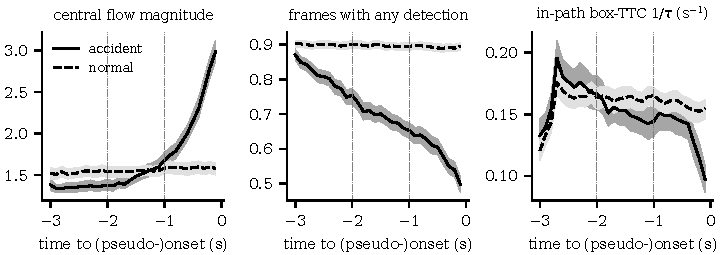
\includegraphics[width=\textwidth]{figures/fig_dynamics.pdf}
\caption{Event-aligned means with bootstrap 95\% bands for accident clips (solid) and normal clips (dashed, aligned to a pseudo-onset). Dotted lines mark the window boundaries}
\label{fig:dynamics}
\end{figure}

\subsection{Cost and Camera-Observable Context}
Per frame on a laptop RTX~4060 GPU, detection with tracking takes \RtDetect~ms, scene descriptors \RtScene~ms, optical flow \RtFlow~ms, lanes \RtLane~ms and kinematics under 1~ms, in total \RtTotal~ms or about \RtFPS{} frames per second, the frame rate of CCD. As a bound on what a forward camera could supply, XGBoost on 51,641 U.S. police-reported crashes (CRSS 2024~\cite{crss2026}; target: suspected serious or fatal injury, 11.2\% prevalence, injury-derived inputs removed) reaches a test AUC of 0.612 (95\% CI [0.595, 0.631]) from context alone, 0.684 [0.668, 0.701] with the road-user and vehicle types a camera could observe (paired $\Delta$AUC $+0.072$, 95\% CI [0.058, 0.088]) and 0.763 [0.749, 0.775] with the full report; camera-observable context thus recovers about 70\% of the full report's above-chance discrimination. The variables are police-coded, so this is an upper bound for perception.

%=============================================================================
\section{Discussion and Limitations}
%=============================================================================
The main finding is methodological: on CCD, accident and normal clips differ in how they were recorded and encoded, so crash-versus-normal AP, however high, mostly measures the source, and a transparent baseline makes this visible because the scene cues alone reproduce most of the score. Within accident clips, box-growth TTC from a generic detector does not signal the approaching accident while detection coverage falls, whereas detector-free flow cues do. (An early prototype trained on synthetic labels that were a formula of the inputs showed a fusion gain that merely reproduced the label generator, which motivated our real-label, clip-level protocol.)

\paragraph{Limitations.} The within-accident task asks whether the last second differs from earlier frames of the same clip, not whether a clip would have ended in an accident, and it does not estimate false alarms on normal driving, for which a source-matched normal set is needed. CCD clips last 5~s, which caps lead time. We did not separate detector from tracker losses, so the coverage collapse may be tracker-specific, and box-growth TTC was not validated against measured range. Each model was trained once. CRSS is U.S.\ police-coded data, and dense, unmarked Indian traffic is rare in CCD.

%=============================================================================
\section{Conclusion}
%=============================================================================
DriveSense is a transparent baseline for single-dashcam collision anticipation: calibration-free time-to-contact from boxes and from flow divergence, scene and motion cues, gradient-boosted fusion with TreeSHAP attributions, and a protocol that splits by clip, fixes thresholds on held-out clips and tests for source leakage. Encoding properties alone separate CCD's accident and normal clips, so crash-versus-normal scores are unreliable evidence of anticipation; within accident clips the fused cues reach an AUC of \WFusedAUC, with flow and detection coverage carrying the signal that box-growth TTC lacks.

\paragraph{Data and Code Availability.} CCD~\cite{bao2020} and CRSS~\cite{crss2026} are publicly available from their providers. All feature-extraction, analysis and evaluation scripts, the per-clip feature tables and the full robustness-slice and operating-curve tables (CSV) are available in the authors' public repository \texttt{sidii1/DriveSense} on GitHub.

%=============================================================================
\begin{thebibliography}{99}
%=============================================================================
\bibitem{who2023} World Health Organization: Global Status Report on Road Safety 2023. World Health Organization, Geneva (2023)

\bibitem{chan2016} Chan, F.-H., Chen, Y.-T., Xiang, Y., Sun, M.: Anticipating accidents in dashcam videos. In: Lai, S.-H., Lepetit, V., Nishino, K., Sato, Y. (eds.) ACCV 2016. LNCS, vol. 10114, pp. 136--153. Springer, Cham (2017). doi:10.1007/978-3-319-54190-7\_9

\bibitem{suzuki2018} Suzuki, T., Kataoka, H., Aoki, Y., Satoh, Y.: Anticipating traffic accidents with adaptive loss and large-scale incident DB. In: Proceedings of the IEEE/CVF Conference on Computer Vision and Pattern Recognition (CVPR), pp. 3521--3529 (2018)

\bibitem{bao2020} Bao, W., Yu, Q., Kong, Y.: Uncertainty-based traffic accident anticipation with spatio-temporal relational learning. In: Proceedings of the 28th ACM International Conference on Multimedia, pp. 2682--2690. ACM, New York (2020). doi:10.1145/3394171.3413827

\bibitem{torralba2011} Torralba, A., Efros, A.A.: Unbiased look at dataset bias. In: Proceedings of the IEEE Conference on Computer Vision and Pattern Recognition (CVPR), pp. 1521--1528 (2011). doi:10.1109/CVPR.2011.5995347

\bibitem{geirhos2020} Geirhos, R., Jacobsen, J.-H., Michaelis, C., Zemel, R., Brendel, W., Bethge, M., Wichmann, F.A.: Shortcut learning in deep neural networks. Nature Machine Intelligence \textbf{2}(11), 665--673 (2020). doi:10.1038/s42256-020-00257-z

\bibitem{lundberg2017} Lundberg, S.M., Lee, S.-I.: A unified approach to interpreting model predictions. In: Advances in Neural Information Processing Systems 30 (NIPS 2017), pp. 4765--4774 (2017)

\bibitem{lundberg2020} Lundberg, S.M., Erion, G., Chen, H., DeGrave, A., Prutkin, J.M., Nair, B., et al.: From local explanations to global understanding with explainable AI for trees. Nature Machine Intelligence \textbf{2}(1), 56--67 (2020). doi:10.1038/s42256-019-0138-9

\bibitem{yao2023} Yao, Y., Wang, X., Xu, M., Pu, Z., Wang, Y., Atkins, E., Crandall, D.J.: DoTA: unsupervised detection of traffic anomaly in driving videos. IEEE Transactions on Pattern Analysis and Machine Intelligence \textbf{45}(1), 444--459 (2023). doi:10.1109/TPAMI.2022.3150763

\bibitem{lee1976} Lee, D.N.: A theory of visual control of braking based on information about time-to-collision. Perception \textbf{5}(4), 437--459 (1976). doi:10.1068/p050437

\bibitem{dagan2004} Dagan, E., Mano, O., Stein, G.P., Shashua, A.: Forward collision warning with a single camera. In: Proceedings of the IEEE Intelligent Vehicles Symposium, pp. 37--42. IEEE (2004)

\bibitem{yolov8} Jocher, G., Chaurasia, A., Qiu, J.: Ultralytics YOLOv8, version 8.0.0. Software (2023)

\bibitem{zhang2022} Zhang, Y., Sun, P., Jiang, Y., Yu, D., Weng, F., Yuan, Z., et al.: ByteTrack: multi-object tracking by associating every detection box. In: Avidan, S., et al. (eds.) ECCV 2022. LNCS, vol. 13682, pp. 1--21. Springer, Cham (2022). doi:10.1007/978-3-031-20047-2\_1

\bibitem{chen2016} Chen, T., Guestrin, C.: XGBoost: a scalable tree boosting system. In: Proceedings of the 22nd ACM SIGKDD International Conference on Knowledge Discovery and Data Mining, pp. 785--794. ACM, New York (2016). doi:10.1145/2939672.2939785

\bibitem{farneback2003} Farneb\"ack, G.: Two-frame motion estimation based on polynomial expansion. In: Bigun, J., Gustavsson, T. (eds.) SCIA 2003. LNCS, vol. 2749, pp. 363--370. Springer, Heidelberg (2003). doi:10.1007/3-540-45103-X\_50

\bibitem{yu2020} Yu, F., Chen, H., Wang, X., Xian, W., Chen, Y., Liu, F., et al.: BDD100K: a diverse driving dataset for heterogeneous multitask learning. In: Proceedings of the IEEE/CVF Conference on Computer Vision and Pattern Recognition (CVPR), pp. 2633--2642 (2020). doi:10.1109/CVPR42600.2020.00271

\bibitem{holm1979} Holm, S.: A simple sequentially rejective multiple test procedure. Scandinavian Journal of Statistics \textbf{6}(2), 65--70 (1979)

\bibitem{efron1993} Efron, B., Tibshirani, R.J.: An Introduction to the Bootstrap. Chapman \& Hall/CRC, New York (1993). doi:10.1201/9780429246593

\bibitem{crss2026} National Center for Statistics and Analysis: Crash Report Sampling System Analytical User's Manual, 2016--2024. Report No. DOT HS 813 796. National Highway Traffic Safety Administration, Washington, DC (2026). doi:10.21949/krxa-cb93

\end{thebibliography}
\end{document}
